\documentclass{amsart}
\usepackage{tikz, mathpazo}
\linespread{1.2}
\title{Problem Set 4}
\begin{document}
\maketitle
\subsection*{Question 1 (7 Marks, 2014 Exam)}

Each of seven students has chosen three courses from ten options, and must sit an exam for each of his or her three choices.  Two students sitting the same exam must do so at the same time, but no student can sit more than one exam in the same day.  The table of choices is given below:$$\begin{array}{cc|cc}
\text{student} & \text{Exams} & \text{student} & \text{Exams}  \\
A & 1,2,3 & E & 6,8,10 \\
B & 1,4,5 & F & 7,8,9 \\
C & 2,4,6 & G & 1,9,10 \\
D & 3,5,7 & &
\end{array}$$ Explain how to relate this question to a graph $G$ so that the chromatic number of $G$ is the smallest number of days required to schedule the exams.  Find this number; you should give an example of a schedule with that number of days and explain why it cannot be done with fewer.

\begin{proof}
  We construct a graph $G$ so that the vertices are the exams, and there is an edge between two exams if there is a student taking both exams.  Then if we take the colours to be the possible exam dates, we see that a vertex colouring of $G$ is equivalent to an admissible exam schedule, and so $\chi(G)$ gives the smallest number of days required to schedule the exams.  The graph $G$ is shown below.
 

  
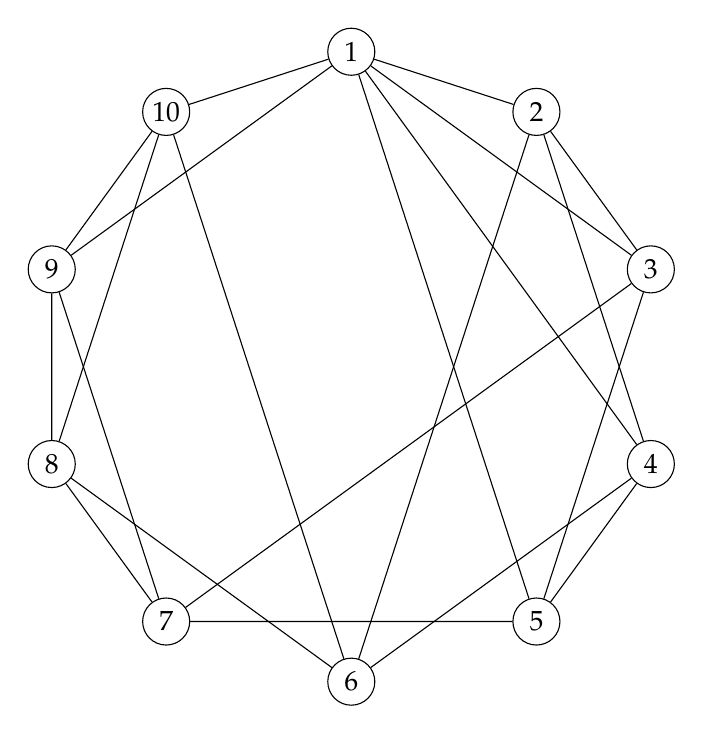
\begin{tikzpicture}
\tikzstyle{vertex}=[circle, draw, minimum size=17pt, inner sep=0pt]

\foreach \x in {1,2,...,10} {
\node[vertex] (\x) at (126-\x*36:4cm) {\x};
}
\draw (1)--(2)--(3)--(1)--(4)--(5)--(1)--(9)--(10)--(1);
\draw (6)--(2)--(4)--(6)--(8)--(10)--(6);
\draw (7)--(8)--(9)--(7)--(3)--(5)--(7);

\end{tikzpicture}

We see $G$ has triangles, so $\chi(G)\geq 3$.  Trying to colour $G$ with three colours, 1,2,3 must be three different colours, without loss of generality 1 is Red, 2 is Blue, and 3 is Green.  Then
\begin{itemize}
\item Using triangle 1,2,4, we see 4 must be green.
\item Using triangle 1,3,5, we see 5 must be blue.
\item Using triangle 2,4,6, we see 6 must be red
\item Using triangle 3,5,7, we see 7 must be red
\end{itemize}

Now 8,9 and 10 must all be different colours as they are a triangle.  But none of them can be red: 8 is adjacent to 6 and 7, which are red, and 9 and 10 are adjacent to 1, which is red.  Therefore, $\chi(G)>3$.

It is not hard to colour $G$ with 4 colours, however: in our attempt at colouring them above, 8,9 and 10 are *only* adjacent to red vertices, so we can make 8 blue, 9 green, and 10 a fourth colour, say yellow.  This would give the corresponding schedule:
$$\begin{array}{c|c}
  \text{Day 1 (red)} & 1, 6,7 \\
  \text{Day 2 (blue)} & 2,5,8 \\
  \text{Day 3 (Green)} & 3, 4, 9 \\
  \text{Day 4 (Yellow)} & 10
  \end{array}$$
though many other schedules are possible.



  \end{proof}

\section*{Question 2 (4 marks, 2014 exam)}

Define the \emph{chromatic index} of a graph.  What is the chromatic index of the graph shown:
 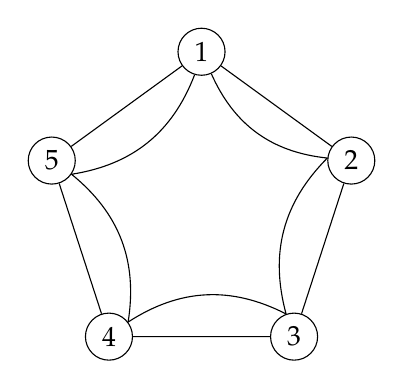
\begin{tikzpicture}
\tikzstyle{vertex}=[circle, draw, minimum size=17pt, inner sep=0pt]

\foreach \x in {1,2,...,5} {
\node[vertex] (\x) at (162-\x*72:2cm) {\x};
}  
\draw (1) to[bend right] (2) to[bend right](3) to[bend right](4) to[bend right](5) to[bend right](1);
\draw (1) to (2) to (3) to (4) to(5) to (1);

\end{tikzpicture}

 \begin{proof}
   The chromatic index $\chi^\prime(G)$ of a graph $G$ is the fewest number of colours needed to colour the eges of $G$ so that edges that share a vertex have different colours.

   In the graph $G$ shown, every vertex has at least degree four, and so at least four colours are necessary -- the four edges touching 1 must all be different.  Let's try to colour the edges with four colours.  Without loss of generality the two edges between 1 and 2 are red and blue, and the two edges between 1 and 5 are green and yellow.  Then the two edges between 2 and 3 must also be green and yellow, and the two edges between 3 and 4 must be red and blue, but now an edge between 4 and 5 cannot be red, blue, green or yellow, and so we see $\chi^\prime(G)>4$.

   By Vizing's theorem we know then that $\chi^\prime(G)=5$, but it is best to illustrate a colouring with 5 colours; one attractive way to do this is to colour the ``inner'' and ``outer'' five cycles with the same five colours in the same order, but shifted slightly.  In other words something like the following, where we have also used the number 1-5 as our colours:

   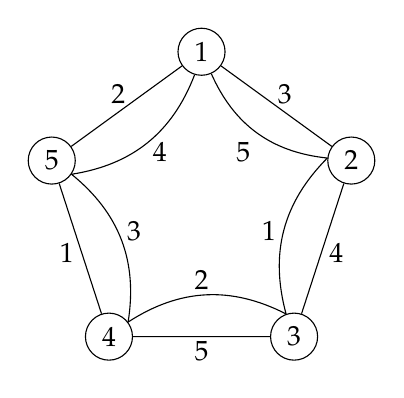
\begin{tikzpicture}
\tikzstyle{vertex}=[circle, draw, minimum size=17pt, inner sep=0pt]

\foreach \x in {1,2,...,5} {
\node[vertex] (\x) at (162-\x*72:2cm) {\x};
}  
\draw (1) to[bend right] (2) to[bend right](3) to[bend right](4) to[bend right](5) to[bend right](1);
\draw (1) to (2) to (3) to (4) to (5) to (1);

\foreach \x in {1,2,...,5} {
\node (\x) at (54-\x*72:.9cm) {\x};
}
\foreach \x in {1,2,...,5} {
\node (\x) at (-90-\x*72:1.8cm) {\x};
}

    \end{tikzpicture}   

 \end{proof}

 \section*{Question 3 14 points}

 \subsection*{Part 1 (4 points)}
 Define the chromatic polynomial $P_\Gamma(k)$ of a graph $\Gamma$.  Explain how to determine the number of vertices, the number of edges, and the chromatic number of $\Gamma$ from the chromatic polynomial.

 \begin{proof}
   The chromatic polynomial $P_\Gamma(k)$ is the number of ways to colour the vertices of $\Gamma$ with $k$ colours so that adjacent vertices have different colours.
   The number of vertices of $\Gamma$ is the degree of $P_\Gamma(k)$, and the number of edges is the negative of the next leading coefficient.  In other words, if $n$ is the number of vertices in $\Gamma$, and $m$ is the number of edges, then
   $$P_\Gamma(k)=k^n-mk^{n-1}+\text{lower order terms}$$
  The chromatic number $\chi(\Gamma)$ is the least number $k$ so that $P_\Gamma(k)\neq 0$. 
   \end{proof}
 
 \subsection*{Part 2 (5 points)}

 State the deletion-contraction relation for $P_G(k)$, and use it prove that $P_G(k)$ is indeed a polynomial.

 \begin{proof}
   The deletion-contraction relation states that if $e$ is an edge in $G$, then

   $$P_G(k)=P_{G\setminus e}(k)-P_{G/e}(k)$$
   where $G\setminus e$ is $G$ with the edge $e$ deleted and $G/e$ is $G$ with the edge $e$ contracted to a vertex.

   To prove that $P_G(k)$ is a polynomial, we induct on the number of edges in $G$.  As a base case, if $G$ has no edges and $n$ vertices, then it is the empty graph $E_n$, and $P_{E_n}(k)=k^n$ as we can colour each of the $n$ vertices independently.

   For the inductive step, assume that $G$ has $m>0$ edges, and that we know that for every graph with less than $m$ edges $P_G(k)$ is a polynomial.  Let $e$ be any edge of $G$.  By deletion contraction we have that
   $$P_G(k)=P_{G\setminus e}(k)-P_{G/e}(k)$$
but since $G\setminus e$ and $G/e$ we know by the inductive hypothesis that both terms on the right hand side are polynomials, and hence $P_G(k)$ is a polynomial.
 \end{proof}
 \subsection*{Part 3 (5 points)}
 Determine the chromatic polynomial of the graph $H$ below:
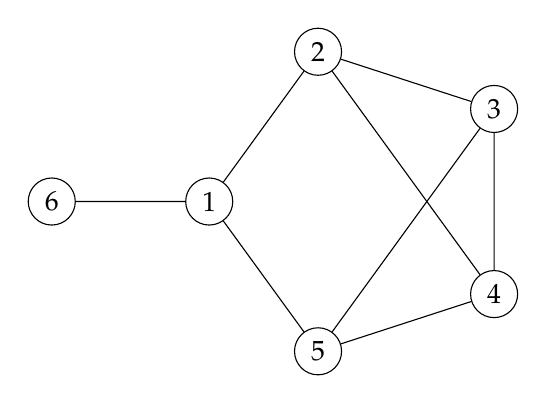
\begin{tikzpicture}[rotate=90]
 \tikzstyle{vertex}=[circle, draw, minimum size=17pt, inner sep=0pt]
\foreach \x in {1,2,...,5} {
\node[vertex] (\x) at (162-\x*72:2cm) {\x};
}  
\node[vertex] (6) at (0,4) {6};
\draw (6)--(1)--(2)--(3)--(4)--(5)--(1);
\draw (2)--(4);
\draw (3)--(5);
\end{tikzpicture}

\begin{proof}
  One way is to use deletion contraction on the edge $e$ between 1 and 2.  If we delete this edge, then colouring vertex by vertex from, say, vertex 2, there are $k$ ways to colour vertex 2, k-1 ways to colour 3, k-2 ways to colour 4 and then 5, and the k-1 ways to colour 1 and 6, giving $P_{H\setminus e}(k)=k(k-1)^3(k-2)^2$.

  On the other hand, if we contract the edge $e$ between 1 and 2, we get a $K_4$ with on extra vertex attached by a single edge, and one can see colouring vertex by vertex or by the gluing formula that this has $P_{H/e}(k)=k(k-1)^2(k-2)(k-3)$.

  Hence
  \begin{align*} P_H(k) &= P_{H\setminus e}(k)-P_{H/e}(k) \\
    &=k(k-1)^3(k-2)^2-k(k-1)^2(k-2)(k-3) \\
    &=k(k-1)^2(k-2)\left[(k-1)(k-2)-(k-3)\right] \\
    &=k(k-1)^2(k-2)(k^2-4k+5)
  \end{align*}

  Another way is by case by case analysis: either vertices 2 and 5 have the same colour, or they have different colours.

If vertices 2 and 5 have different colours, then vertices 2-5 form a $K_4$, and there are $k(k-1)(k-2)(k-3)$ ways to colour them, then there are $k-2$ ways to colour vertex 1 and $k-1$ ways to colour vertex 6, giving $k(k-1)^2(k-2)^2(k-3)$ colourings in this case.
  
  If vertices 2 and 5 have the same colour, there are $k$ ways to choose that colour, then $(k-1)$ ways to colour, in order, vertices 1, 6, and 3, and finally $k-2$ ways to colour vertex 4, giving $k(k-1)^3(k-2)$ colourings in this case.

  Adding the cases, we have

  \begin{align*} P_H(k) &=k(k-1)^2(k-2)^2(k-3) + k(k-1)^3(k-2) \\
    &=k(k-1)^2(k-2)\left[(k-2)(k-3)+(k-1)\right] \\
    &=k(k-1)^2(k-2)(k^2-4k+5)
    \end{align*}
 



  \end{proof}



\end{document}
